\section{Activity selection problem} 
We would like to book as many pairwise disjoint activities as possible for a seminar/lecture room.
Each activity is characterized by two features : its starting time and its finishing time. Let us write the $i$-th activity as $a_i = [s_i \: \:  f_i[$ with $s_i$ and $f_i$ its starting and finishing time, respectively. Let us also assume that activities are sorted such that $f_1 \leq f_2 \leq \ldots \leq f_n$.

\begin{figure}[h!]
\centering
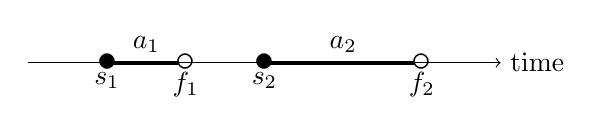
\begin{tikzpicture}

\draw[->] (0,0) -> (6,0);

\draw (1,0) node{{\Large $\bullet$}} node[below]{$s_1$};
\draw (2,0) node{{\Large$\circ$}} node[below]{$f_1$};
\draw[ultra thick] (1,0) -> (1.9,0);
\draw (1.5,0) node[above]{$a_1$};

\draw (3,0) node{{\Large $\bullet$}} node[below]{$s_2$};
\draw (5,0) node{{\Large$\circ$}} node[below]{$f_2$};
\draw[ultra thick] (3,0) -> (4.9,0);
\draw (4,0) node[above]{$a_2$};

\draw (6,0) node[right]{time};
\end{tikzpicture}
\caption{Example of two disjoint activities}
\end{figure}

\subsection{Dynamic programming solution}
\subsubsection{Can we divide this into subproblems ?}

Let us define $S_{ij} = \{ a_k \: | \: a_k \subseteq [f_i \: \: s_j [ \: \}$ and $c_{ij}$ as the maximum number of disjoint activities we can book in $[f_i \: \: s_j [$  from activities in $S_{ij}$.

\begin{figure}[h!]
\centering
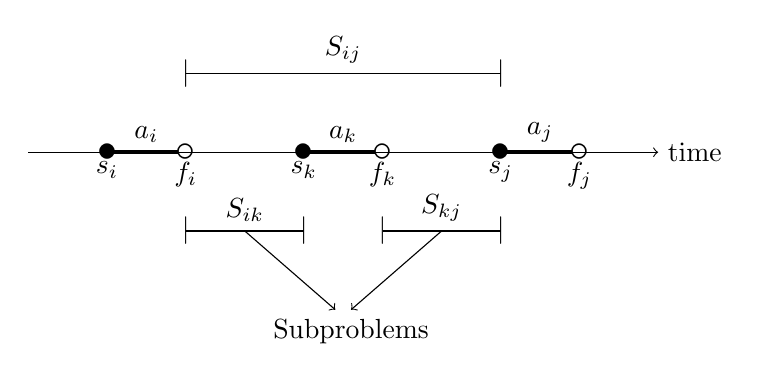
\begin{tikzpicture}

\draw[->] (0,0) -> (8,0);
\draw (8,0) node[right]{time};

\draw (1,0) node{{\Large $\bullet$}} node[below]{$s_i$};
\draw (2,0) node{{\Large$\circ$}} node[below]{$f_i$};
\draw[ultra thick] (1,0) -> (1.9,0);
\draw (1.5,0) node[above]{$a_i$};

\draw (3.5,0) node{{\Large $\bullet$}} node[below]{$s_k$};
\draw (4.5,0) node{{\Large$\circ$}} node[below]{$f_k$};
\draw[ultra thick] (3.5,0) -> (4.4,0);
\draw (4,0) node[above]{$a_k$};

\draw (6,0) node{{\Large $\bullet$}} node[below]{$s_j$};
\draw (7,0) node{{\Large$\circ$}} node[below]{$f_j$};
\draw[ultra thick] (6,0) -> (6.9,0);
\draw (6.5,0) node[above]{$a_j$};

\draw (2,1) -> (6,1);
\draw (2,1) node{$|$};
\draw (6,1) node{$|$};
\draw (4,1) node[above]{$S_{ij}$};

\draw (2,-1) -> (3.5,-1);
\draw (2,-1) node{$|$};
\draw (3.5,-1) node{$|$};
\draw (2.75,-1) node[above]{$S_{ik}$};

\draw (4.5,-1) -> (6,-1);
\draw (4.5,-1) node{$|$};
\draw (6,-1) node{$|$};
\draw (5.25,-1) node[above]{$S_{kj}$};

\draw[->] (2.75,-1) -> (3.9,-2);
\draw[->] (5.25,-1) -> (4.1,-2);
\draw (4.1,-2) node[below]{Subproblems};

\end{tikzpicture}
\caption{Decomposition in subproblems}
\label{Subproblems}
\end{figure}

From Figure \ref{Subproblems}, it is pretty easy to see that
\begin{equation*}
c_{ij} = \left\lbrace
\begin{tabular}{cl}
$\max \limits_{a_k \in S_{ij}} (c_{ik} +c_{kj}+1)$ & if $S_{ij} \neq \emptyset$  \\
$0$ & if $S_{ij} = \emptyset$ .
\end{tabular} \right.
\end{equation*}
This decomposition in subproblems tells us that there exists a dynamic programming algorithm to solve the activity selection problem.

\subsection{Greedy solution}
However, we can be smarter than that ! Indeed, we can know which activity to choose in advance : the one that finishes first among $S_{ij}$, i.e. the one with smalllest index in $S_{ij}$ (since $f_1 \leq f_2 \leq \ldots \leq f_n$).


\subsubsection{Why ?}

If we have an optimal solution (for the subproblem $c_{ij}$) that doesn’t use $a_{k_{\text{min}}}$ (the activity in $S_{ij}$ with earliest finish) but starts with $a_k \in S_{ij}$ instead, then we can get a solution just as good (same cardinality $c_{ij}$) by replacing $a_k$ with $a_{k_{\text{min}}}$. This is illustrated on Figure \ref{Illustration argument greedy}.


\begin{figure}[h!]
\centering
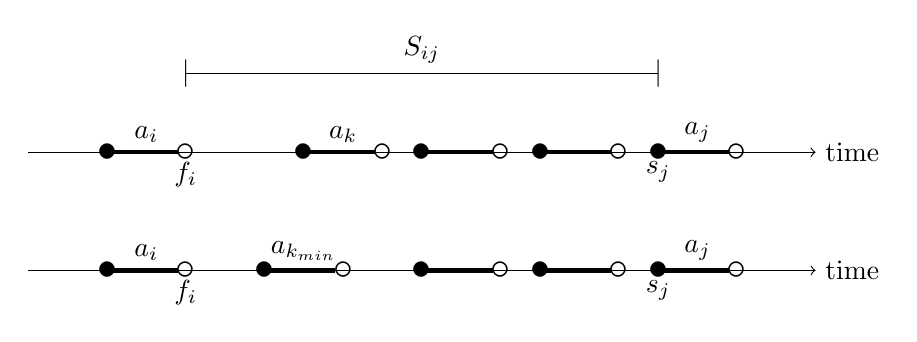
\begin{tikzpicture}

\draw[->] (0,0) -> (10,0);
\draw (10,0) node[right]{time};

\draw (1,0) node{{\Large $\bullet$}};
\draw (2,0) node{{\Large$\circ$}} node[below]{$f_i$};
\draw[ultra thick] (1,0) -> (1.9,0);
\draw (1.5,0) node[above]{$a_i$};

\draw (3.5,0) node{{\Large $\bullet$}};
\draw (4.5,0) node{{\Large$\circ$}};
\draw[ultra thick] (3.5,0) -> (4.4,0);
\draw (4,0) node[above]{$a_k$};

\draw (5,0) node{{\Large $\bullet$}};
\draw (6,0) node{{\Large$\circ$}};
\draw[ultra thick] (5,0) -> (5.9,0);

\draw (6.5,0) node{{\Large $\bullet$}};
\draw (7.5,0) node{{\Large$\circ$}};
\draw[ultra thick] (6.5,0) -> (7.4,0);

\draw (8,0) node{{\Large $\bullet$}} node[below]{$s_j$};
\draw (9,0) node{{\Large$\circ$}};
\draw[ultra thick] (8,0) -> (8.9,0);
\draw (8.5,0) node[above]{$a_j$};

\draw (2,1) -> (8,1);
\draw (2,1) node{$|$};
\draw (8,1) node{$|$};
\draw (5,1) node[above]{$S_{ij}$};



\draw[->] (0,-1.5) -> (10,-1.5);
\draw (10,-1.5) node[right]{time};

\draw (1,-1.5) node{{\Large $\bullet$}};
\draw (2,-1.5) node{{\Large$\circ$}} node[below]{$f_i$};
\draw[ultra thick] (1,-1.5) -> (1.9,-1.5);
\draw (1.5,-1.5) node[above]{$a_i$};

\draw (3,-1.5) node{{\Large $\bullet$}};
\draw (4,-1.5) node{{\Large$\circ$}};
\draw[ultra thick] (3,-1.5) -> (3.9,-1.5);
\draw (3.5,-1.5) node[above]{$a_{k_{\text{min}}}$};

\draw (5,-1.5) node{{\Large $\bullet$}};
\draw (6,-1.5) node{{\Large$\circ$}};
\draw[ultra thick] (5,-1.5) -> (5.9,-1.5);

\draw (6.5,-1.5) node{{\Large $\bullet$}};
\draw (7.5,-1.5) node{{\Large$\circ$}};
\draw[ultra thick] (6.5,-1.5) -> (7.4,-1.5);

\draw (8,-1.5) node{{\Large $\bullet$}} node[below]{$s_j$};
\draw (9,-1.5) node{{\Large$\circ$}};
\draw[ultra thick] (8,-1.5) -> (8.9,-1.5);
\draw (8.5,-1.5) node[above]{$a_j$};

\end{tikzpicture}
\caption{Illustration of the greedy algorithm argument}
\label{Illustration argument greedy}
\end{figure}

Consequently, a greedy algorithm can be designed to take advantage of that fact. That greedy algorithm is the following :
\begin{lstlisting}[label={list:c6:activitySelectionGreedy},caption=Pseudo-code of the greedy algorithm for activity selection problem]
ActivitySelect({ a_1,...,a_n})
	{a_1} union ActivitySelect({activities disjoint from a_1})
\end{lstlisting}
The time complexity of this algorithm is 
\begin{equation*}
\overbrace{\Theta(n \log n)}^{\text{Sort}} + \: \Theta(n) = \Theta(n \log n) \: .
\end{equation*}
On the other hand, dynamic programming would cost $\mathcal{O}(n^3)$. We can see a big difference in terms of time complexity between the greedy approach and the dynamic programming approach for the activity selection problem.

“Greedy” : we build up a solution from $\emptyset$ by adding at each step the “best” piece. In a short-sighted way, we don’t care for the future.

A greedy approach can sometimes be adopted in dynamic programming situations where the \textbf{principle of suboptimality} applies. However, a greedy choice does not always exist. 

\subsubsection{Other examples of greedy algorithms}
\begin{itemize}
 \item Minimum spanning tree : Kruskal and Prim algorithms
 \item Shortest path : Dijkstra algorithm
\end{itemize}

\section{Scheduling problem}
Let us now consider another famous problem:
\begin{itemize}
 \item $n$ jobs, each having a one unit of time duration
 \item $t_i$: deadline for the job $i$
 \item $c_i$: profit for job $i$
\end{itemize}

It is important to say that we earn $c_i$ from job $i$ if and only if it is scheduled to finish before its deadline $t_i$. The aim is to maximize the total profit $P_{Total}$, being the sum of the individual profits of the jobs finishing before their respective deadline.

\subsection{Example}
Let's take the following instance
\begin{table}[h!]
\centering
\begin{tabular}{c|cccc}
$i$ & 1 & 2 & 3 & 4 \\
\hline $c_i$ & 50 & 10 & 15 & 30 \\
$t_i$ & 2 & 1 & 2 & 1
\end{tabular}
\end{table} ~\\
One possible scheduling of the jobs is the following
\begin{figure}[h!]
\centering

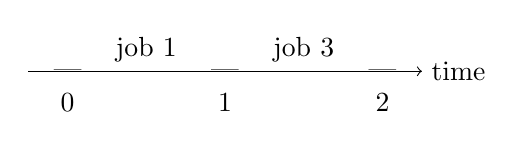
\begin{tikzpicture}
\draw[->] (0,0) -> (5,0) node[right]{time};
\draw (0.5,0) node{|};
\draw (2.5,0) node{|};
\draw (4.5,0) node{|};

\draw (0.5,-0.4) node{0};
\draw (2.5,-0.4) node{1};
\draw (4.5,-0.4) node{2};

\draw (1.5,0) node[above]{job 1};
\draw (3.5,0) node[above]{job 3};
\end{tikzpicture}

\end{figure} ~\\
In that particular case, the total profit will simply be
\begin{equation*}
P_{Total} = c_1 + c_3 = 50 +15 = 65 \: .
\end{equation*}
Another possible scheduling of the jobs is
\begin{figure}[h!]
\centering

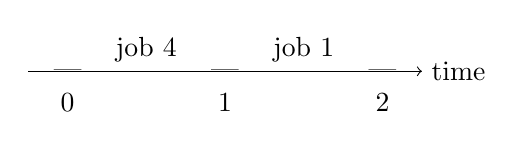
\begin{tikzpicture}
\draw[->] (0,0) -> (5,0) node[right]{time};
\draw (0.5,0) node{|};
\draw (2.5,0) node{|};
\draw (4.5,0) node{|};

\draw (0.5,-0.4) node{0};
\draw (2.5,-0.4) node{1};
\draw (4.5,-0.4) node{2};

\draw (1.5,0) node[above]{job 4};
\draw (3.5,0) node[above]{job 1};
\end{tikzpicture}

\end{figure} ~\\
We have now improved the total profit:
\begin{equation*}
P_{Total} = c_1 + c_4 = 50 + 30 = 80 \: .
\end{equation*}
This is in fact the optimal solution. Indeed, if we schedule first job 4, and then job 1, we obtain the best solution since they are the jobs with highest individual profits, and furthermore it is impossible to schedule more than 2 jobs, then it must be the best combination.


% ----------------------------------------------------------------------
%
% ----------------------------------------------------------------------

\subsection{Generalization: Greedy Algorithm}

The greedy algorithm is very simple:

% , with index = deadlines: i=1,2,3,...
\begin{lstlisting}[label={list:c6:SchedulingGreedy},caption=Pseudo-code of the greedy algorithm for scheduling problem]
L = Empty list % will hold selected jobs
S = stack of jobs ordered by profit with highest on top.
While S not Empty
	a = S.pop()
	Try add a in L at the farthest time index within deadlines
\end{lstlisting}

The list \texttt{L} has length $T$ where $T$ is the time horizon considered. The $i$-th element of \texttt{L} is the job being scheduled from $t = i-1$ to $t = i$, or is empty if no job is scheduled at that time slot. Note that this algorithm works if $t_i \in \mathbb{N} \: \: \forall i$ but doesn’t work if there exist a $t_i$ non-integral. Let's see how it works on our example (in this case $T = 2$):

\begin{lstlisting}[label={list:c6:SchedulingGreedy_Example},caption=Example of the greedy algorithm for scheduling problem]
Select job with highest profit : job1
	Try add job1 in L -> possible
	$ L ={/, job1} : Profit of 50
Select job with 2nd highest profit : job4
	Try add job4 in L -> possible
	$ L ={job4, job1} : Profit of 80
Select job with 3rd highest profit : job3
	Try add job3 in L -> impossible
	$ Do not add it
Select with 4th highest profit : job2
	Try add job2 in L -> impossible
	$ Do not add it
STOP
\end{lstlisting}

\subsection{Does the greedy algorithm work? How to check that a set of jobs is feasible?}
\begin{theorem}
A set of jobs with deadlines $ t_1 \leq t_2  \leq \hdots \leq t_n $ is feasible, if and only if, the order $1, 2, \ldots, n$ is feasible.
\end{theorem}
\begin{proof} ~

\begin{itemize}
\item ($\Rightarrow$) If the schedule

\begin{figure}[h!]
\centering

\begin{tikzpicture}
\draw[->] node[above left]{jobs} (0,0) -> (6,0) node[right]{time};

\draw (1,0) node{|};
\draw (2,0) node{|};
\draw (1.5,0) node[above]{$j$};
\draw (2,-0.4) node{$a$};

\draw (4,0) node{|};
\draw (5,0) node{|};
\draw (4.5,0) node[above]{$i$};
\draw (5,-0.4) node{$b$};

\end{tikzpicture}

\end{figure}
is feasible, with $t_i \leq t_j$, then we can swap $i$ and $j$, and it’s still a feasible schedule. Indeed, since this schedule is feasible, we have $t_i  \geq b$ and $t_j \geq a$. Furthermore, we have that $b \geq a$ and $t_j \geq t_i$. It follows that $t_i \geq b \geq a$ and $t_j \geq t_i \geq b$, which make the schedule where $i$ and $j$ are swapped feasible. We can repeat swaps as many times as necessary $ \Rightarrow$ order $1,2,\hdots, n$ feasible.

\item ($\Leftarrow$) Trivial.
\end{itemize}

\end{proof}

Note that if the jobs are already ordered by increasing deadlines, then checking feasibility of the schedule is done in $\Theta(n)$.

\begin{theorem}
The greedy algorithm provides the optimal scheduling.
\end{theorem}

\begin{proof}
Suppose that $I = \{ i_1, i_2, \hdots, i_n \}$ is the greedy solution and
$J = \{j_1,j_2, \ldots , j_m \}$ is the optimal solution.
$\Rightarrow$ Both feasible $\Rightarrow$ can be ordered at unit time slots from the left


\begin{figure}[h!]
\centering

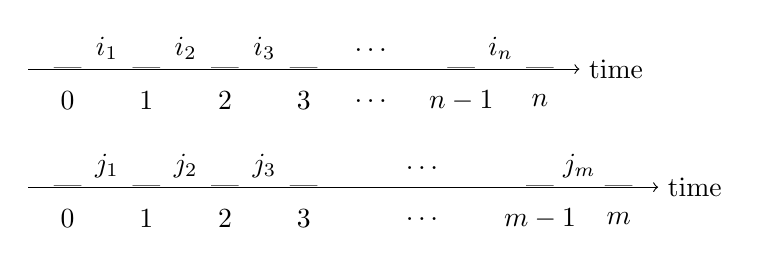
\begin{tikzpicture}
\draw[->] (0,0) -> (7,0) node[right]{time};

\draw (0.5,0) node{|};
\draw (1.5,0) node{|};
\draw (2.5,0) node{|};
\draw (3.5,0) node{|};

\draw (5.5,0) node{|};
\draw (6.5,0) node{|};

\draw (0.5,-0.4) node{0};
\draw (1.5,-0.4) node{1};
\draw (2.5,-0.4) node{2};
\draw (3.5,-0.4) node{3};
\draw (5.5,-0.4) node{$n-1$};
\draw (6.5,-0.4) node{$n$};

\draw (1,0) node[above]{$i_1$};
\draw (2,0) node[above]{$i_2$};
\draw (3,0) node[above]{$i_3$};
\draw (6,0) node[above]{$i_n$};

\draw (4.35,0.1) node[above]{$\ldots$};
\draw (4.35,-0.4) node{$\ldots$};



\draw[->] (0,-1.5) -> (8,-1.5) node[right]{time};

\draw (0.5,-1.5) node{|};
\draw (1.5,-1.5) node{|};
\draw (2.5,-1.5) node{|};
\draw (3.5,-1.5) node{|};

\draw (6.5,-1.5) node{|};
\draw (7.5,-1.5) node{|};

\draw (0.5,-1.9) node{0};
\draw (1.5,-1.9) node{1};
\draw (2.5,-1.9) node{2};
\draw (3.5,-1.9) node{3};
\draw (6.5,-1.9) node{$m-1$};
\draw (7.5,-1.9) node{$m$};

\draw (1,-1.5) node[above]{$j_1$};
\draw (2,-1.5) node[above]{$j_2$};
\draw (3,-1.5) node[above]{$j_3$};
\draw (7,-1.5) node[above]{$j_m$};

\draw (5,-1.4) node[above]{$\ldots$};
\draw (5,-1.9) node{$\ldots$};



\end{tikzpicture}

\end{figure}

We want to “align” $I$ and $J$ as much as possible to compare them: schedule same jobs at the same time.

\begin{example}
\begin{leftbar}
Suppose that job $k \in I \bigcap J$, e.g. $k = i_4 = j_8$, then job $k$ is scheduled at the 4-th time slot in $I$ and at the 8-th time slot in $J$. We want to swap jobs either in $I$ or in $J$ in order to have job $k$ scheduled at the same time slot in both schedules. \\

To that end, we will swap $i_4$ and $i_8$ in $I$. If $i_8$ is empty, then after the swap is performed, $i_4$ will be empty and $i_8$ will contain job $k$. If $i_8 = \tilde{k}$ was not empty, then after the swap has been performed, job $\tilde{k}$ is now scheduled on the 4-th time slot and job $k$ on the 8-th. Moving job $\tilde{k}$ from the 8-th time slot to the 4-th does not put the feasibility of the new schedule in jeopardy, since it is now scheduled earlier. Furthermore, scheduling the job $k$ at the 8-th time slot instead of the 4-th is also feasible since job $k$ is scheduled at that 8-th time slot in $J$, and $J$ is assumed to be feasible. \\

Could we have swapped $j_8$ and $j_4$ in $J$ instead of swapping $i_4$ and $i_8$ in $I$? The answer is : it depends, but in general \textbf{NO} ! Indeed, although scheduling job $k$ at the 4-th time slot instead of at the 8-th in $J$ would always be feasible, there is no guarantee that the job that was initially in $j_4$ would still be feasible at the 8-th time slot, therefore preventing the "swapped" schedule to be feasible !
e.g. : $k = i_7 = j_2$ : then swap $j_2$ and $j_7$. Job $k$ will never be rescheduled
\end{leftbar}
\end{example}

Repeat all swaps until no more is possible, then all common jobs are aligned.
Now, let us take a look at all the situations one could think of where the jobs are different in $I$ and in $J$. The first situation looks like

\begin{figure}[h!]
\centering

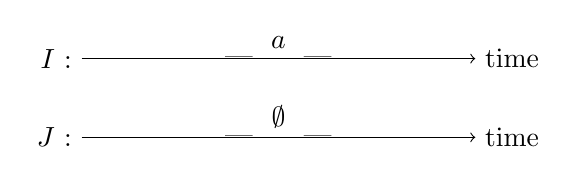
\begin{tikzpicture}
\draw[->] node[left]{$I$ : } (0,0) -> (5,0) node[right]{time};

\draw (2,0) node{|};
\draw (3,0) node{|};
\draw (2.5,0) node[above]{$a$};


\draw[->] (0,-1) node[left]{$J$ : } -> (5,-1) node[right]{time};

\draw (2,-1) node{|};
\draw (3,-1) node{|};
\draw (2.5,-1) node[above]{$\emptyset$};

\end{tikzpicture}

\end{figure}

This first situation is impossible because since $a \notin J$, we can schedule it in the empty slot and improve the total profit of the sequence $J$ strictly. A second situtation is

\begin{figure}[h!]
\centering

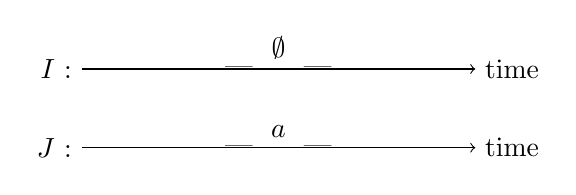
\begin{tikzpicture}
\draw[->] node[left]{$I$ : } (0,0) -> (5,0) node[right]{time};

\draw (2,0) node{|};
\draw (3,0) node{|};
\draw (2.5,0) node[above]{$\emptyset$};


\draw[->] (0,-1) node[left]{$J$ : } -> (5,-1) node[right]{time};

\draw (2,-1) node{|};
\draw (3,-1) node{|};
\draw (2.5,-1) node[above]{$a$};

\end{tikzpicture}

\end{figure}

Once again, this situation is impossible because since $a \notin I$, then adding $a$ to $I$ is feasible $\Rightarrow$ the greedy algorithm would have chosen it. Finally, the last situation that could potentially occur is

\begin{figure}[h!]
\centering

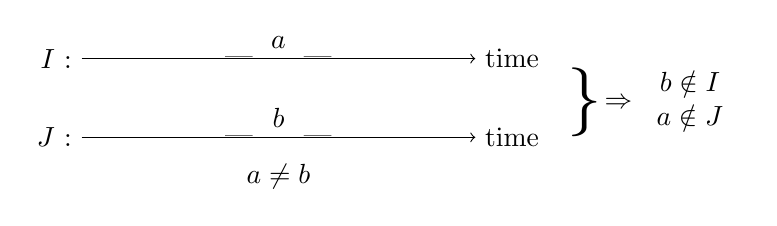
\begin{tikzpicture}
\draw[->] node[left]{$I$ : } (0,0) -> (5,0) node[right]{time};

\draw (2,0) node{|};
\draw (3,0) node{|};
\draw (2.5,0) node[above]{$a$};


\draw[->] (0,-1) node[left]{$J$ : } -> (5,-1) node[right]{time};

\draw (2,-1) node{|};
\draw (3,-1) node{|};
\draw (2.5,-1) node[above]{$b$};

\draw (2.5,-1.5) node{$a \neq b$};
\draw (6,-0.55) node[right]{{\Huge $\left. \right\rbrace$}};
\draw (7.5,-0.55) node{$\Rightarrow \begin{tabular}{c}
$b \notin I$ \\
$a \notin J$
\end{tabular}$};

\end{tikzpicture}

\end{figure}

If $c_b > c_a$ : then the greedy algorithm would have chosen $b$ before $a$ $\Rightarrow b$ would be in $I$. \\
If $c_a > c_b$ : then $J$ is strictly improved by replacing $b$ with $a$, then impossible case. \\
It follows that $c_a = c_b$, and consequently we have that $C_I = C_J$.

\end{proof}

Time complexity 
$\underbrace{\Theta(n \log n)}_{\text{Sort by profit}} + \underbrace{\Theta(n^2 \log n)}_{\text{Sort by deadline $n$ times}}$

But we can do better : $\Theta(n \log n)$
